\chapter{Results}

\section{Dense Object Nets}

For benchmarking, 48GB VRAM GPU is used. As per the VRAM availability, the \ac{ResNet} architecture with pixelwise distribution and pixelwise nt-xent loss are evaluated
with 2048 correspondences for an image pair with the descriptor dimension $D=3$ and batch size of 2. Additionally, both the loss functions are benchmarked with 512 correspondences
for an image pair with descriptor dimension $D=16$ and batch size of 2. Each model is trained for 100 epochs with Adam optimizer~\cite{kingma2014adam} initialized
with learning rate of $3 \times 10^{-5}$ with weight regularization of $1 \times 10^{-4}$. Minimum validation loss is monitored to save best model.
Each epoch took $45s$. Training \ac{DON} with the pixelwise distribution loss occupies less VRAM compared to the pixelwise nt-xent loss.\\

The $PCK@k$ metric Equation \ref{eqn:pck} is computed following the procedure described in \cite{adrian2022efficient}.
The benchmark results are presented in Table~\ref{table:auc_don}, where the numbers in bold
mark the optimal benchmark result ($\uparrow$ signifies higher score is better). The optimal benchmark result is decided based minimum validation loss and computation costs.\\

The results have higher values compared to benchmarking results in preceeding \cite{adrian2022efficient} as the model is evaluated for a single object scene
rather than for a multi-object scene as described in \cite{adrian2022efficient}. The pixelwise distribution loss outperforms the pixelwise contrastive loss for a single object scene in accordance to the
benchmarks in \cite{adrian2022efficient}.

\begin{table}[htb]
    \centering
    \begin{tabular}{lccccc}
        \hline
        \multicolumn{5}{c}{Benchmarking DON for $AUC \pm \sigma \ for \ PCK@K$ $\uparrow$}                                                                                                                 \\ \hline
        \multicolumn{1}{c}{Loss Functions}         & \multicolumn{1}{c|}{D}  & \multicolumn{1}{c}{\ac{ResNet}-18}      & \multicolumn{1}{c}{\ac{ResNet}-34}      & \multicolumn{1}{c}{\ac{ResNet}-50}      \\ \hline
        \multicolumn{1}{l}{Pixelwise Distribution} & \multicolumn{1}{l|}{3}  & \multicolumn{1}{c}{$\mathbf{0.9800}$}   & \multicolumn{1}{c}{$0.9800$}            & \multicolumn{1}{c}{$0.9800$}            \\
        \multicolumn{1}{l}{Pixelwise Distribution} & \multicolumn{1}{l|}{16} & \multicolumn{1}{c}{$0.9800$}            & \multicolumn{1}{c}{$0.9800$}            & \multicolumn{1}{c}{$0.9800$}            \\
        \multicolumn{1}{l}{Pixelwise NT-Xent}      & \multicolumn{1}{l|}{3}  & \multicolumn{1}{c}{$0.9791 \pm 0.0003$} & \multicolumn{1}{c}{$0.9796 \pm 0.0003$} & \multicolumn{1}{c}{$0.9798 \pm 0.0001$} \\
        \multicolumn{1}{l}{Pixelwise NT-Xent}      & \multicolumn{1}{l|}{16} & \multicolumn{1}{c}{$0.9799 \pm 0.0005$} & \multicolumn{1}{c}{$\mathbf{0.9800}$}   & \multicolumn{1}{c}{$0.9776 \pm 0.0039$} \\ \hline
    \end{tabular}
    \caption{DON evaluation against $AUC \pm \sigma \ for \ PCK@K$ metric.}
    \label{table:auc_don}
\end{table}


\begin{table}[htb]
    \centering
    \begin{tabular}{lc}
        \hline
        \multicolumn{2}{c}{Visual Inspection of Descriptor Image}                                                                                                            \\ \hline
        \multicolumn{1}{c|}{Pixelwise distribution loss }                                         & \multicolumn{1}{c}{Pixelwise NT-Xent loss}                               \\
        \multicolumn{1}{c|}{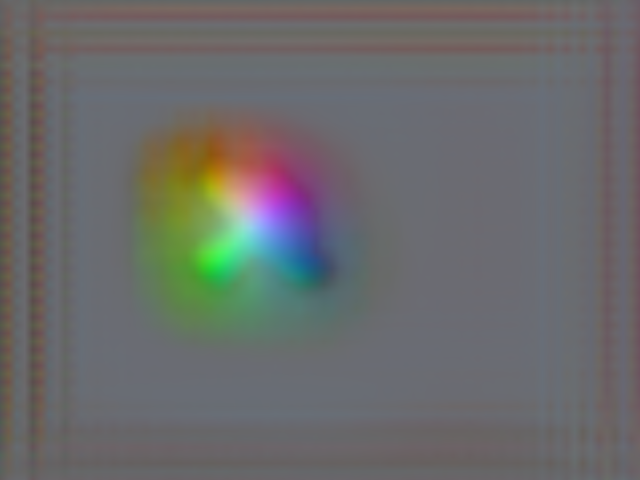
\includegraphics[scale=0.2]{images/don/don-d3-resnet50-nc1024-c.png}} & \multicolumn{1}{c}{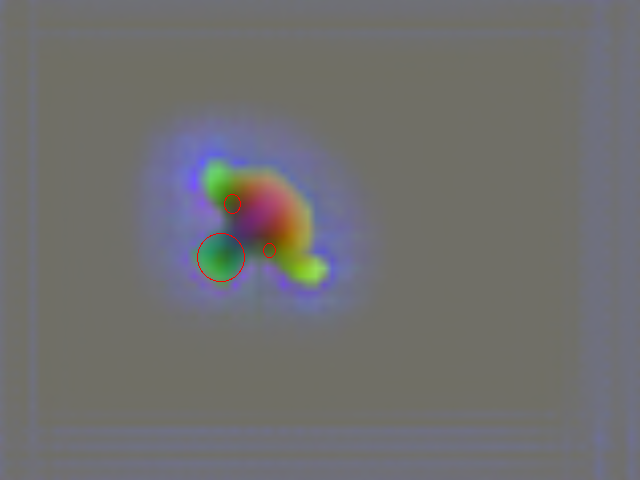
\includegraphics[scale=0.2]{images/don/defects.png} } \\ \hline
    \end{tabular}
    \caption{Visual inspection for optimal placement of descriptors.}
    \label{table:don}
\end{table}

As for the descriptor dimension $D=3$ the pixelwise distribution loss produces consistent results, as described in Table~\ref{table:auc_don}, it is evident that the pixelwise distribution loss produces
optimal descriptors with respect to keypoint spatial expectation compared to the pixelwise nt-xent loss and is chosen for further implementation.\\

To compare both the loss
functions visually, the dense descriptor image is extracted from the \ac{DON} and color encoded by scaling the descriptor ($d \in \mathbb{R}^3$) to the pixel space of $p \in \mathbb{R}^3, \ac{s.t.} \ p \in [0, 255]$. By definition, the dense descriptors are locally
unique to each other. As described in Table~\ref{table:don}, the descriptors encoded by the network trained on the pixelwise nt-xent loss yields the non-optimal descriptors (annotated in red circles in the right image)
compared to the network trained on pixelwise distribution loss which performs better.


\subsection{Manual Method for Robot Grasp Generation}

In the interactive application developed, the descriptors are selected manually. The manually selected descriptors pixels locations are projected to camera frame using depth and camera intrinsics to
produce a 6D pose computed via \ac{PCA}. The \ac{DON} produces consistent descriptors against color jitter, occlusion, illumination and viewpoint detailed in Table~\ref{table:robust_descriptors}. Furthermore, the
6D pose generated via the interactive application is not benchmarked as it is developed to test the consistency of the descriptors produced by \ac{DON} addtionally, the pose produced by \ac{PCA} has different
basis compared to poses present in the dataset.

\begin{table}[htb]
    \centering
    \begin{tabular}{lccccc}
        \hline
        \multicolumn{3}{c}{Illustration of Robust Descriptors}                                                                                                                                                                         \\ \hline
        \multicolumn{1}{c}{Color Jitter}                                       & \multicolumn{1}{c}{Illumination Changes}                               & \multicolumn{1}{c}{Occlusions}                                               \\
        \multicolumn{1}{c}{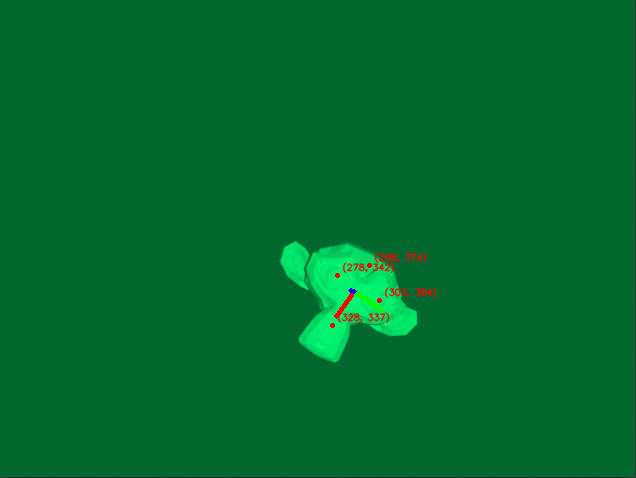
\includegraphics[scale=0.15]{images/don/color.png}} & \multicolumn{1}{c}{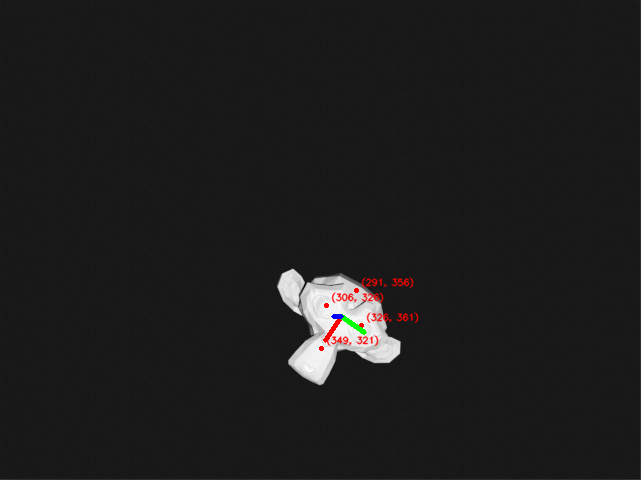
\includegraphics[scale=0.15]{images/don/illum.png}} & \multicolumn{1}{c}{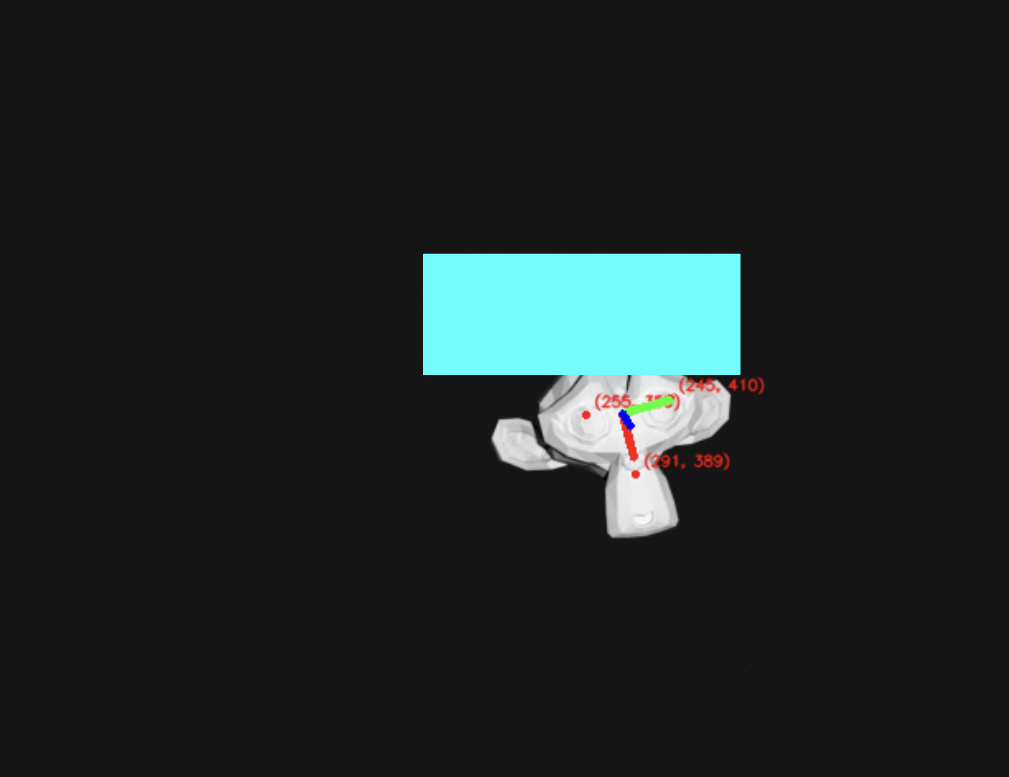
\includegraphics[scale=0.0915]{images/don/occlusion.png}} \\ \hline
    \end{tabular}
    \caption{Testing descriptors for robost 6D pose generation.}
    \label{table:robust_descriptors}
\end{table}








\section{KeypointNet}
\label{subsection:KeypointNet}

The \ac{ResNet} architecture is used to train KeypointNet task for 1000 epochs with batch size 16.
To train the network, ADAM optimizer is used with the learning rate of $1 \times 10^{-3}$ with no weight regularization. The optimal weights to compute
to weighted sum loss in Equation \ref{eqn: weighted_sum} in page \pageref{eqn: weighted_sum} is set to $W=[1.0, 0.2, 1.0, 1.0, 0.0001]^T$. The \ac{ResNet}-18 and \ac{ResNet}-34 architectures are
trained to predict 8, 16, 32 number of geometrically consistent keypoints with $\delta$ = 10 pixel spacing margin. The models are saved monitoring the minimum validation loss while training.\\

To benchmark the KeypointNet, the losses used to train the network itself is applied as it captures information like multiview consistency, relative pose, and whether a keypoint belongs to an object silhoutte, which are the pivotal properties that a keypoint must carry. The Table~\ref{table:keypointnet_benchmark} describes the benchmarking results sampled from 10 random image pairs.
($\downarrow$ in the Table~\ref{table:keypointnet_benchmark} represents that lower score is better.) \\


\begin{table}[htb]
    \centering
    \begin{tabular}{lccccc}
        \hline
        \multicolumn{6}{c}{KeypointNet Benchmarking $\downarrow$}                                                                                                                                                                             \\ \hline
        \multicolumn{1}{c}{Model}          & \multicolumn{1}{c|}{N}  & \multicolumn{1}{c}{$\mathcal{L}_{mc}$}  & \multicolumn{1}{c}{$\mathcal{L}_{pose}$} & \multicolumn{1}{c}{$\mathcal{L}_{obj}$} & \multicolumn{1}{c}{$\mathcal{L}_{sep}$} \\
        \multicolumn{1}{l}{\ac{ResNet}-18} & \multicolumn{1}{l|}{8}  & \multicolumn{1}{c}{$0.1720 \pm 0.0545$} & \multicolumn{1}{c}{$0.0826 \pm 0.1123$}  & \multicolumn{1}{c}{$0 \pm 0$}           & \multicolumn{1}{c}{$0 \pm 0$}           \\
        \multicolumn{1}{l}{\ac{ResNet}-34} & \multicolumn{1}{l|}{8}  & \multicolumn{1}{c}{$0.1115 \pm 0.0244$} & \multicolumn{1}{c}{$0.1303 \pm 0.1325$}  & \multicolumn{1}{c}{$0 \pm 0$}           & \multicolumn{1}{c}{$0.0084 \pm 0.0465$} \\
        \multicolumn{1}{l}{\ac{ResNet}-18} & \multicolumn{1}{l|}{16} & \multicolumn{1}{c}{$0.2121 \pm 0.0676$} & \multicolumn{1}{c}{$0.1427 \pm 0.1332$}  & \multicolumn{1}{c}{$0 \pm 0$}           & \multicolumn{1}{c}{$0.2745 \pm 0.0576$} \\
        \multicolumn{1}{l}{\ac{ResNet}-34} & \multicolumn{1}{l|}{16} & \multicolumn{1}{c}{$0.0830 \pm 0.0891$} & \multicolumn{1}{c}{$0.0732 \pm 0.0891$}  & \multicolumn{1}{c}{$0.1813 \pm 0.2142$} & \multicolumn{1}{c}{$0 \pm 0$}           \\
        \multicolumn{1}{l}{\ac{ResNet}-18} & \multicolumn{1}{l|}{32} & \multicolumn{1}{c}{$1.0130 \pm 0.2978$} & \multicolumn{1}{c}{$0.0990 \pm 0.1276$}  & \multicolumn{1}{c}{$1.3405 \pm 0.3274$} & \multicolumn{1}{c}{$0.0088 \pm 0.0234$} \\
        \multicolumn{1}{l}{\ac{ResNet}-34} & \multicolumn{1}{l|}{32} & \multicolumn{1}{c}{$0.4206 \pm 0.1906$} & \multicolumn{1}{c}{$0.0974 \pm 0.0990$}  & \multicolumn{1}{c}{$0.0928 \pm 0.2440$} & \multicolumn{1}{c}{$0.0122 \pm 0.0508$} \\
        \multicolumn{1}{l}{\ac{ResNet}-50} & \multicolumn{1}{l|}{32} & \multicolumn{1}{c}{$0.1983 \pm 0.6378$} & \multicolumn{1}{c}{$0.1312 \pm 0.1262$}  & \multicolumn{1}{c}{$1.3815 \pm 0$}      & \multicolumn{1}{c}{$0.2019 \pm 0.0829$} \\ \hline
    \end{tabular}
    \caption{Benchmarking KeypointNet with individual losses.}
    \label{table:keypointnet_benchmark}
\end{table}

As per the benchmarking results in Table~\ref{table:keypointnet_benchmark} in page~\pageref{table:keypointnet_benchmark}, the \ac{ResNet}-34 performs better overall.
As per the \ac{ResNet}-18 training history, the validation loss increases after some epochs and does not predict with consistent lower validation loss while, the \ac{ResNet}-34 yields consistent decreasing in
validation loss till the end of the training refer Figure~\ref{fig:output_keypointnet}.  Additionally, \ac{ResNet}-50 is benchmarked to predict 32 keypoints and found under performing. Hence, \ac{ResNet}-34 architecture instead will be used for future implementation.

\begin{figure}[htb]
    \centering
    \caption{Output of trained \ac{ResNet}-34 for KeypointNet task.}
    \label{fig:output_keypointnet}
    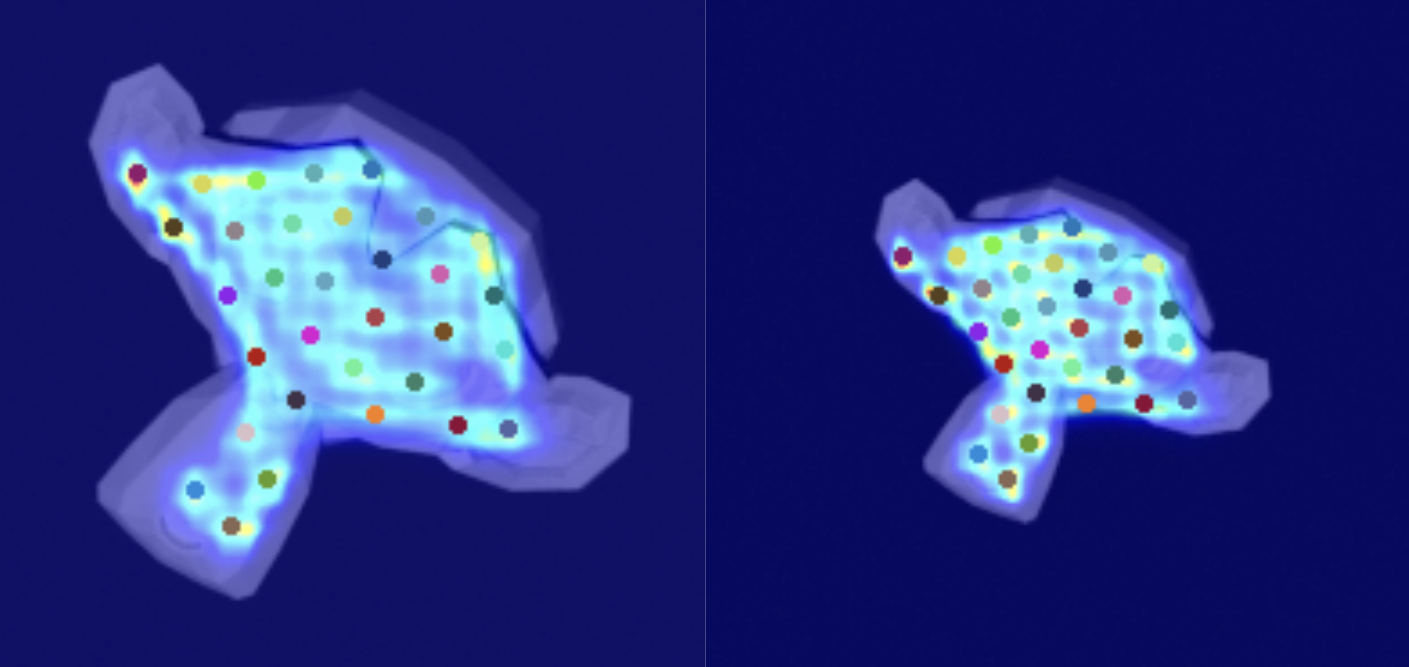
\includegraphics[scale=0.1]{images/keypointnet/output.png}
\end{figure}

\pagebreak





















\section{End-to-End Training}

\subsection{KeypointNet Informed Dense Object Nets}

The \ac{ResNet}-34 is used to implement KeypointNet tasks supplying 256 number of correspondences per image implying 512 correspondences for an image pair to train \ac{ResNet}-18 based \ac{DON} with margin $\delta = 3$ pixel apart.
\ac{DON} is trained with pixelwise distribution loss with the descriptor dimension $D=3$. Adam optimizer is used to train the networks jointly with learning rate of $1 \times 10^{-3}$ and no weight regularization.
$W$ for training the KeypointNet loss is set to the same value as used in KeypointNet benchmarking. The benchmarked results in Table~\ref{table:keypointnet_informed_don_benchmark} in page~\pageref{table:keypointnet_informed_don_benchmark}
are computed by extracting output features from the individual networks stacked to train in end-to-end training fashion.\\

\begin{table}[htb]
    \centering
    \begin{tabular}{lcccc}
        \hline
        \multicolumn{5}{c}{KeypointNet Informed \ac{DON} Benchmarking}                                                                                                                                                              \\ \hline
        \multicolumn{1}{l|}{\ac{DON}}    & \multicolumn{4}{c}{$AUC \pm \sigma \ for \ PCK@K metric$}                                                                                                                                \\
        \multicolumn{1}{l|}{}            & \multicolumn{4}{c}{$0.9666 \pm 0.0034$}                                                                                                                                                  \\ \hline
        \multicolumn{1}{l|}{KeypointNet} & \multicolumn{1}{c}{$\mathcal{L}_{mc}$}                    & \multicolumn{1}{c}{$\mathcal{L}_{pose}$} & \multicolumn{1}{c}{$\mathcal{L}_{obj}$} & \multicolumn{1}{c}{$\mathcal{L}_{sep}$} \\
        \multicolumn{1}{l|}{}            & \multicolumn{1}{c}{$0.4367 \pm 0.9020$}                   & \multicolumn{1}{c}{$0.0893 \pm 0.1897$}  & \multicolumn{1}{c}{$0.0019 \pm 0.0020$} & \multicolumn{1}{c}{$0.0957 \pm 0.0160$} \\ \hline
    \end{tabular}
    \caption{Benchmarking KeypointNet informed \ac{DON} for their individual performance.}
    \label{table:keypointnet_informed_don_benchmark}
\end{table}

The \ac{DON} performance descreases compared to the bechmarking results in Table~\ref{table:auc_don} in page~\pageref{table:auc_don}.
The keypoints computed from the KeypointNet are not consistent as one can see for $ \mathcal{L}_{mc}$ in Table~\ref{table:keypointnet_informed_don_benchmark}.
As the inconsistent keypoints are supplied to \ac{DON} for training, the performance of \ac{DON} decreases. Furthermore, the pixelwise
distribution loss is not robust to inconsistent correspondence as claimed in \cite{florence2020dense}.




























\subsection{Dense Object Nets Informed KeypointNet}

The \ac{ResNet}-18 is used to train \ac{DON} of the descriptor dimension $D=3$ with 256 correspondences per image implying 512 correspondences are sampled to train an image pair.
The \ac{ResNet}-34 is used to train KeypointNet predicting 8 keypoints on dense object representations with $\delta = 10$ pixels apart to pick lables.
ADAM optimizer is used to train the networks jointly with learning rate of $1 \times 10^{-3}$ and no weight regularization.
$W$ for training the KeypointNet loss is set to the same value as used in KeypointNet benchmarking. The benchmarked results in Table~\ref{table:don_informed_informed_benchmark} in page~\pageref{table:don_informed_informed_benchmark}
are computed by extracting output features from the individual networks stacked to train in end-to-end training fashion.

\begin{table}[htb]
    \centering
    \begin{tabular}{lcccc}
        \hline
        \multicolumn{5}{c}{\ac{DON} Informed KeypointNet Benchmarking}                                                                                                                                                              \\ \hline
        \multicolumn{1}{l|}{\ac{DON}}    & \multicolumn{4}{c}{$AUC \pm \sigma \ for \ PCK@K metric$}                                                                                                                                \\
        \multicolumn{1}{l|}{}            & \multicolumn{4}{c}{$0.9756 \pm 0.0005$}                                                                                                                                                  \\ \hline
        \multicolumn{1}{l|}{KeypointNet} & \multicolumn{1}{c}{$\mathcal{L}_{mc}$}                    & \multicolumn{1}{c}{$\mathcal{L}_{pose}$} & \multicolumn{1}{c}{$\mathcal{L}_{obj}$} & \multicolumn{1}{c}{$\mathcal{L}_{sep}$} \\
        \multicolumn{1}{l|}{}            & \multicolumn{1}{c}{$0.4323 \pm 0.1671$}                   & \multicolumn{1}{c}{$0.1048 \pm 0.0476$}  & \multicolumn{1}{c}{$0.0029 \pm 0.0050$} & \multicolumn{1}{c}{$0\pm 0$}            \\ \hline
    \end{tabular}
    \caption{Benchmarking results of \ac{DON} informed KeypointNet with autopicked labels.}
    \label{table:don_informed_informed_benchmark}
\end{table}

As per the benchmarking results in Table~\ref{table:don_informed_informed_benchmark}, the performance of \ac{DON} decreases as the number of correspondences to train the \ac{DON} network is limited to 256 for an image.
This implies that all the loss functions to train the \ac{DON} are sensitive to number of correspondences.\\

The Table~\ref{table:sampled object generalized labels} describes the single class generalized object labels autonomously picked by the KeypointNet from the dense descriptor image. The policy $\pi$ assigns a random
priority to store the labels for `Suzanne' offline. The labels are queried from the descriptor space using 8 keypoints regressed by the KeypointNet with the seperation margin
$\delta = 10$ in pixel space.

\begin{table}[htb]
    \centering
    \begin{tabular}{ll}
        \hline
        \multicolumn{2}{c}{Autosampled single class generalized object label}                     \\ \hline
        \multicolumn{1}{c}{$\pi$(Priority)} & \multicolumn{1}{c}{Label}                           \\ \hline
        \multicolumn{1}{c}{1}               & \multicolumn{1}{c}{$[-3.3778, -3.2668,  6.2417]^T$} \\
        \multicolumn{1}{c}{2}               & \multicolumn{1}{c}{$[-3.4086, -3.3175,  6.2570]^T$} \\
        \multicolumn{1}{c}{3}               & \multicolumn{1}{c}{$[-3.3793, -3.3144,  6.2799]^T$} \\
        \multicolumn{1}{c}{4}               & \multicolumn{1}{c}{$[-3.4003, -3.3314,  6.2663]^T$} \\
        \multicolumn{1}{c}{5}               & \multicolumn{1}{c}{$[-3.3072, -3.1737,  6.1999]^T$} \\
        \multicolumn{1}{c}{6}               & \multicolumn{1}{c}{$[-3.2575, -3.1253,  6.2076]^T$} \\
        \multicolumn{1}{c}{7}               & \multicolumn{1}{c}{$[-3.3644, -3.2777,  6.2714]^T$} \\
        \multicolumn{1}{c}{8}               & \multicolumn{1}{c}{$[-3.3931, -3.2843,  6.2413]^T$} \\ \hline
    \end{tabular}
    \caption{KeypointNet sampled class generalized labels for `Suzanne'.}
    \label{table:sampled object generalized labels}
\end{table}


\subsection{Mining Dense Object Nets Representations in KeypointNet}

The KeypointNet is trained to regress 256 keypoints with $\delta = 2$ using \ac{ResNet}-34 architecture
with the same training setting to benchmark the KeypointNet.
The upsampled dense output feature dimension is reduced to $D=16$ for comparing with the \ac{DON} whose descriptor
dimension is set to $D=16$.\\

The dense representation put forth by the upsampled dense output feature layer is benchmarked against
$PCK@$ as in Equation \ref{eqn:pck} in page~\pageref{eqn:pck}, the same benchmarking process for \ac{DON}.
The upsampled dense output feature evaluates to $AUC \pm \sigma \ for \ PCK@k, \forall k \in [1, 100] = 0.9759 \pm 0.0051$.
This result inlines with the \ac{DON} bechmarked against pixelwise nt-xent loss with descriptor dimension $D = 16$.
Futhermore, the loss for predicting the keypoints increased as illustrated in Figure~\ref{fig:increase_loss_in_keypoints} in page~\pageref{fig:increase_loss_in_keypoints}
as the upsampled dense output feature dimension is reduced from 256 to 16.\\

\begin{figure}[htb]
    \centering
    \caption{Errors in keypoints predictions from KeypointNet modified to benchmark against \ac{DON} representations.}
    \label{fig:increase_loss_in_keypoints}
    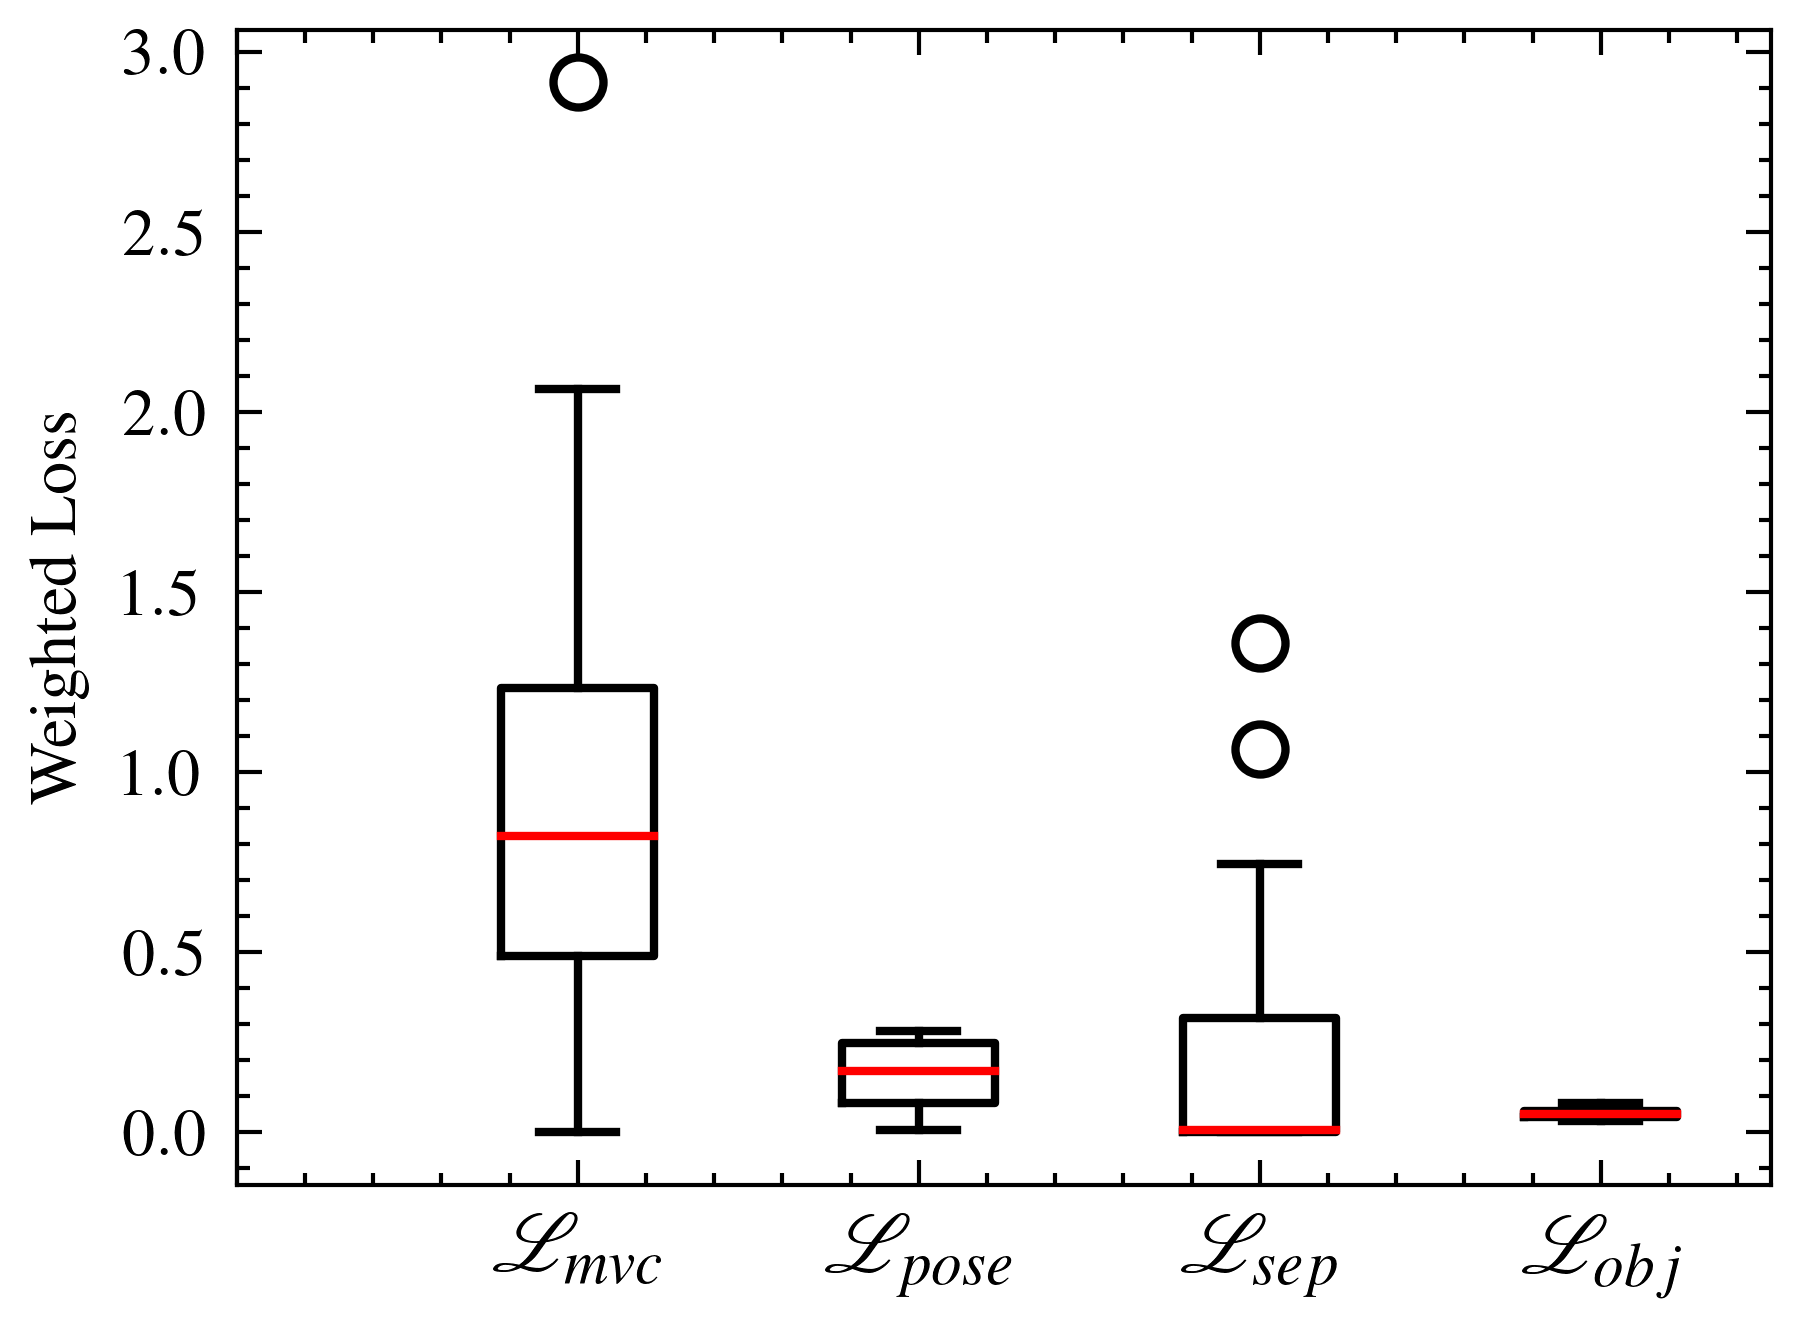
\includegraphics[scale=.75]{images/keypointnet/34-D.png}
\end{figure}


To represent
the descriptor space image of dimension $D = 16$ in an image as in Figure~\ref{fig:descriptors_from_keypointnet}, \ac{PCA} is used to reduce
the dimension to a higher dimensional sub-space of $D = 3$ (a higher dimensional sub-space is the lower dimensional representation of a higher dimension).
\ac{PCA} is only used for visualization purposes. The representation is not consistent as \ac{PCA} preserves variance in the data while
projecting it to a higher dimensional sub-space explaining the ears of `Suzanne' with same color.
No further attempts are carried out to represent dense descriptor images in an image as it does not align with the thesis objective.

\begin{figure}[htb]
    \centering
    \caption{Depiction of dense descriptors extracted from KeypointNet.}
    \label{fig:descriptors_from_keypointnet}
    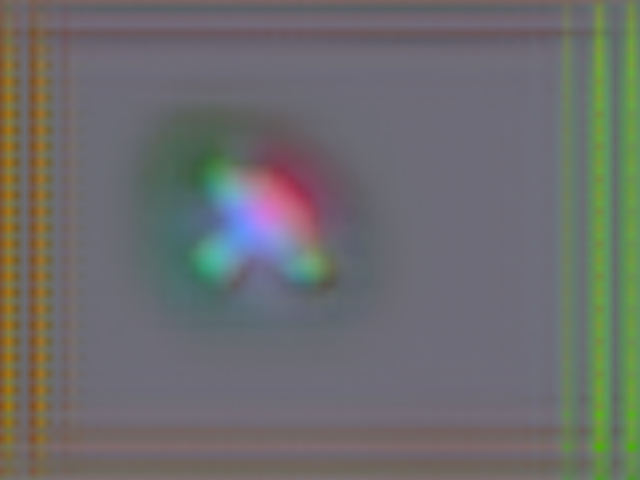
\includegraphics[scale=0.22]{images/don/don-d16-resnet50-nc256-c.png}
\end{figure}





















































\section{Generalizing ``Caps''}

\subsection{Semantic Correspondence Mapping Pipeline}

KeypointNet is trained to predict $100$ keypoints with pixel spacing margin $\delta = 5$. Adam optimizer is used to train
the network for 1000 epochs with a learning rate $1 \times 10^{-3}$ and no weight regularization. The $W$ is set similarly to the same value as in the KeypointNet benchmarking. Furthermore, Keypointnet is based on \ac{ResNet}-34 architecture with upsampled dense output dimension set to $256$.\\

The KeypointNet is benchmarked for its loss function as detailed in  Table~\ref{table:benchmark_semantic_correspondence} in page~\pageref{table:benchmark_semantic_correspondence}. The benchmarking yields higher errors
compared to the results in Table~\ref{table:keypointnet_benchmark} in page~\pageref{table:keypointnet_benchmark} as the number of correspondences is higher and semantically equivalent objects are trained. For the visual inspection purposes, $8$  keypoints are sampled randomly as in the Table~\ref{table:visual_inspection_semantic_correspondence}
in page~\pageref{table:visual_inspection_semantic_correspondence}. Most of the keypoints are semantically well placed, with a few keypoints regressed with high multiview consistent errors.\\


\begin{table}[htb]
    \centering
    \begin{tabular}{lcccc}
        \hline
        \multicolumn{4}{c}{Semantic Correspondence Mapping Pipeline Benchmarking}                                                                                              \\
        \multicolumn{1}{c}{$\mathcal{L}_{mc}$}  & \multicolumn{1}{c}{$\mathcal{L}_{pose}$} & \multicolumn{1}{c}{$\mathcal{L}_{obj}$} & \multicolumn{1}{c}{$\mathcal{L}_{sep}$} \\ \hline
        \multicolumn{1}{c}{$5.1342 \pm 2.8517$} & \multicolumn{1}{c}{$0.1456 \pm 0.0628$}  & \multicolumn{1}{c}{$0.2135 \pm 0.0771$} & \multicolumn{1}{c}{$2.0256 \pm 1.2637$} \\ \hline
    \end{tabular}
    \caption{Benchmarking: KeypointNet used for mapping semantic correspondences.}
    \label{table:benchmark_semantic_correspondence}
\end{table}


\begin{table}[htb]
    \centering
    \begin{tabular}{lcccc}
        \hline
        \multicolumn{3}{c}{Visual Inspection of Semantic Correspondences}                                                                                                                                                           \\ \hline
        \multicolumn{1}{c}{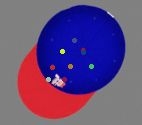
\includegraphics[scale=0.87]{images/cap/image_a.png}} & \multicolumn{1}{c}{\includegraphics[scale=1]{images/cap/image_b.png}} & \multicolumn{1}{c}{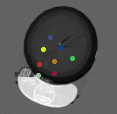
\includegraphics[scale=0.95]{images/cap/image_c.png}} \\ \hline
    \end{tabular}
    \caption{Illustration of semantic correspondences. The semantic correspondences are color coded.}
    \label{table:visual_inspection_semantic_correspondence}
\end{table}

Furthermore, the semantic correspondence pipeline is examined for the root cause of the high errors.
The semantic correspondence pipeline did not converge for a cap in the synthetic dataset.
As illustrated in Figure~\ref{fig:non_convergence} in page~\pageref{fig:non_convergence}, the keypoints do not meet
the properties of geometrically consistent keypoints further, explaining the high errors in Table~\ref{table:benchmark_semantic_correspondence}
in page~\pageref{table:benchmark_semantic_correspondence}. The object is removed from the dataset, and the
semantic correspondence pipeline is trained again to resolve predictions of keypoints with errors.
The errors decrease after another training as seen in Table ~\ref{table:revised_benchmark_semantic_correspondence} in page~\pageref{table:revised_benchmark_semantic_correspondence}.

\begin{figure}[htb]
    \centering
    \caption{Non-Convergence in Semantic Correspondence Pipeline.}
    \label{fig:non_convergence}
    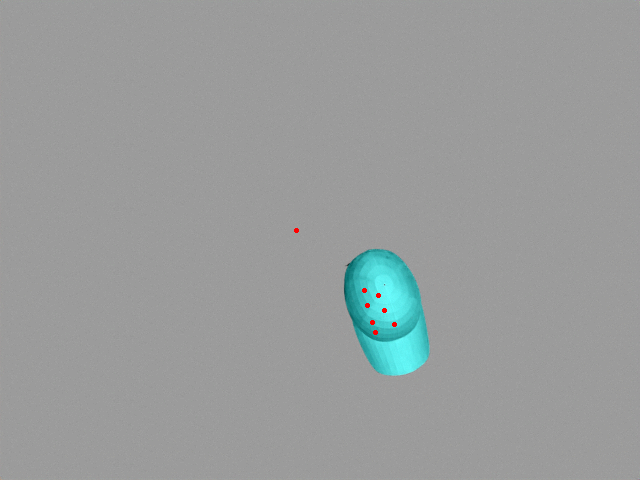
\includegraphics[scale=0.2]{images/cap/defect_a.png}
\end{figure}

\begin{table}[htb]
    \centering
    \begin{tabular}{lcccc}
        \hline
        \multicolumn{4}{c}{Revised Semantic Correspondence Mapping Pipeline Benchmarking}                                                                                      \\ \hline
        \multicolumn{1}{c}{$\mathcal{L}_{mc}$}  & \multicolumn{1}{c}{$\mathcal{L}_{pose}$} & \multicolumn{1}{c}{$\mathcal{L}_{obj}$} & \multicolumn{1}{c}{$\mathcal{L}_{sep}$} \\ \hline
        \multicolumn{1}{c}{$2.1210 \pm 1.5937$} & \multicolumn{1}{c}{$0.0754 \pm 0.1840$}  & \multicolumn{1}{c}{$0.0780 \pm 0.0079$} & \multicolumn{1}{c}{$0.1374 \pm 1.8752$} \\ \hline
    \end{tabular}
    \caption{Revised bechmarking for semantic correspondences mapping pipeline.}
    \label{table:revised_benchmark_semantic_correspondence}
\end{table}


\subsection{Evaluating Single Class Generalized Labels in the Wild}

Two images of caps were collected using a smartphone with a camera to benchmark single-label generalizing ability in the wild as illustrated in Table~\ref{table:cap_wild} in page~\pageref{table:cap_wild}.
Furthermore, from now on, benchmarking method initially used to quantify the neural network tasks will not be used.\\

\begin{table}[htb]
    \centering
    \begin{tabular}{lcccc}
        \hline
        \multicolumn{2}{c}{Caps in the Facility}                                                                                                        \\
        \multicolumn{1}{c}{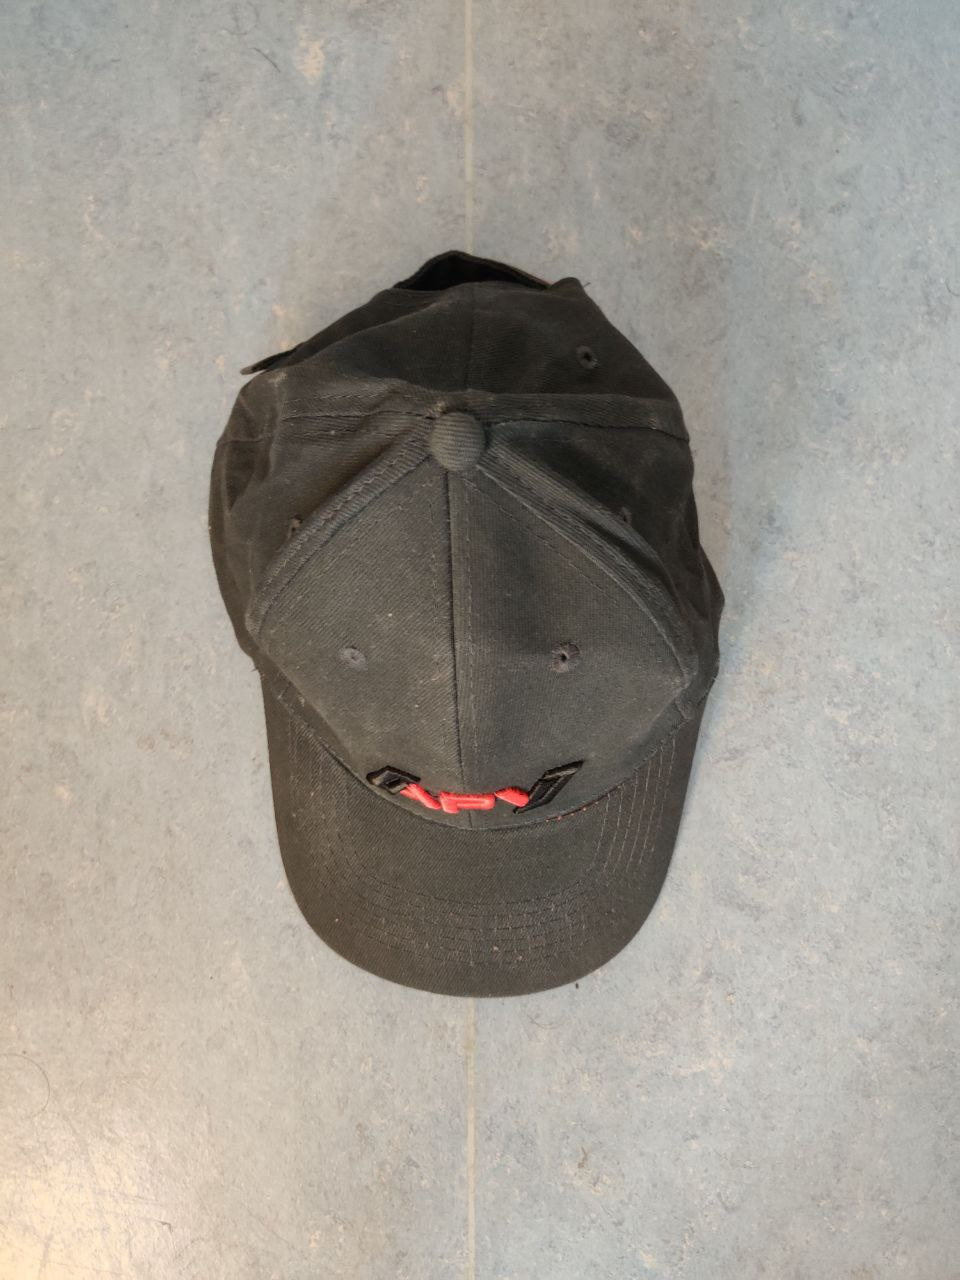
\includegraphics[scale=0.1]{images/cap/wild_a.jpg}} & \multicolumn{1}{c}{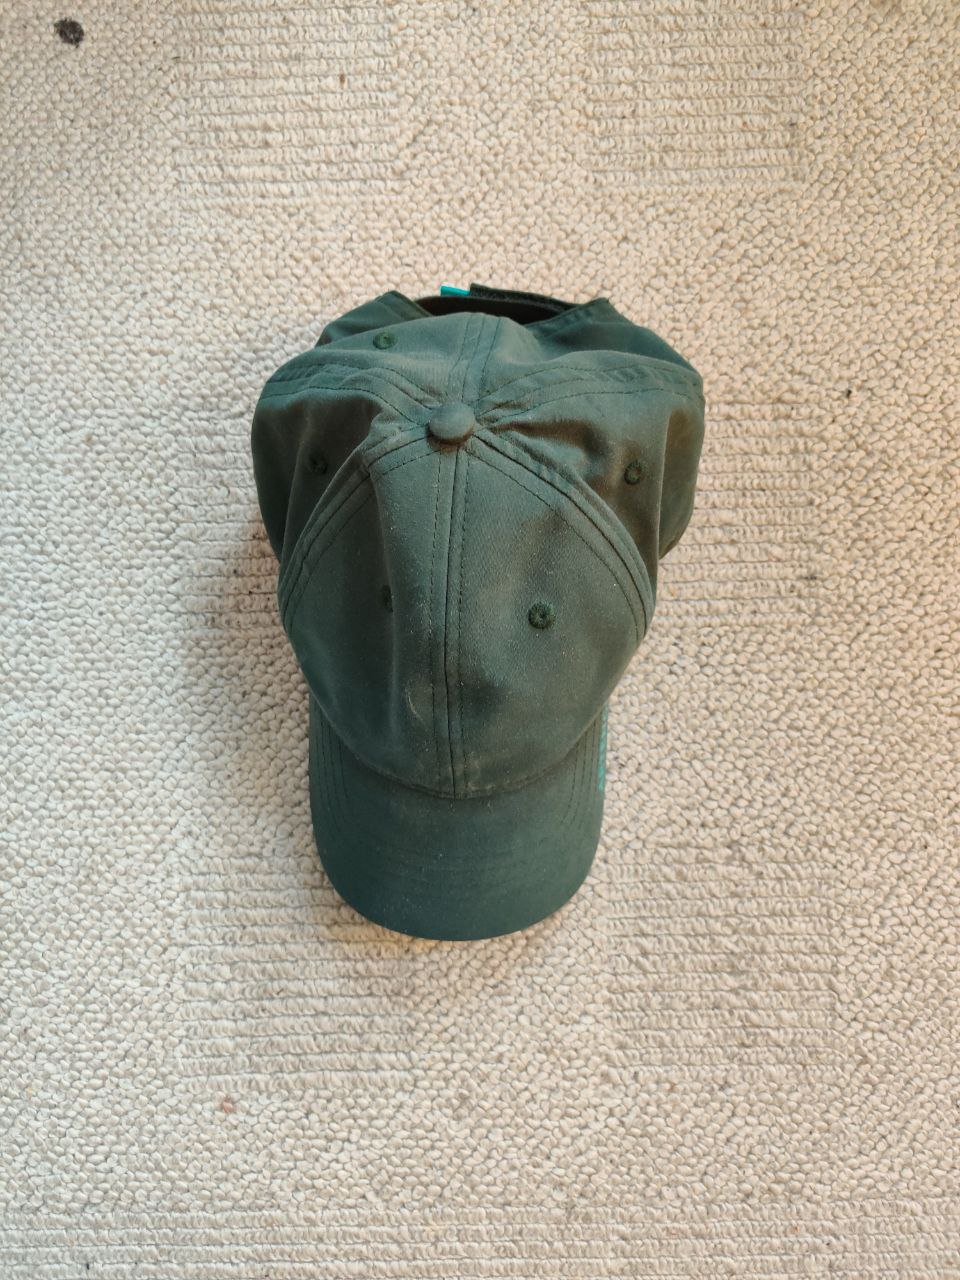
\includegraphics[scale=0.1]{images/cap/wild_b.jpg}} \\ \hline
    \end{tabular}
    \caption{Depiction of two caps found in the facility.}
    \label{table:cap_wild}
\end{table}

For evaluating \ac{DON} trained on the synthetic dataset of caps, \ac{DON} is trained with \ac{ResNet}-34 architecture with pixelwise correspondence loss with the dense
descriptor dimension $D=3$ as it is previously found to be performing optimally as can be seen in Table~\ref{table:auc_don} in page \pageref{table:auc_don} and computationally economical.
Additionally, \ac{DON} is trained on the semantic correspondences supplied from the KeypointNet, and ADAM optimizer is used with a learning rate of $3 \times 10^{-5}$
with weight regularization set to $1 \times 10^{-4}$ for 100 epochs with batch size 2.\\

The trained \ac{DON} is tested on the cap images. Judging from
Figure~\ref{fig:caps_in_wild_testing}, the descriptors are not placed semantically well. The heatmaps in the image describe a descriptor's spatial probability in two images. The heatmaps are generated from the interactive
application developed to generate robot grasps manually with the temperature parameter set to $t=-0.3$ in Gaussian kernel search space Equation \ref{eqn:gaussian_kernel} in
page~\pageref{eqn:gaussian_kernel}.\\

\begin{figure}[htb]
    \centering
    \caption{Testing optimal descriptor placement for the caps in the wild.}
    \label{fig:caps_in_wild_testing}
    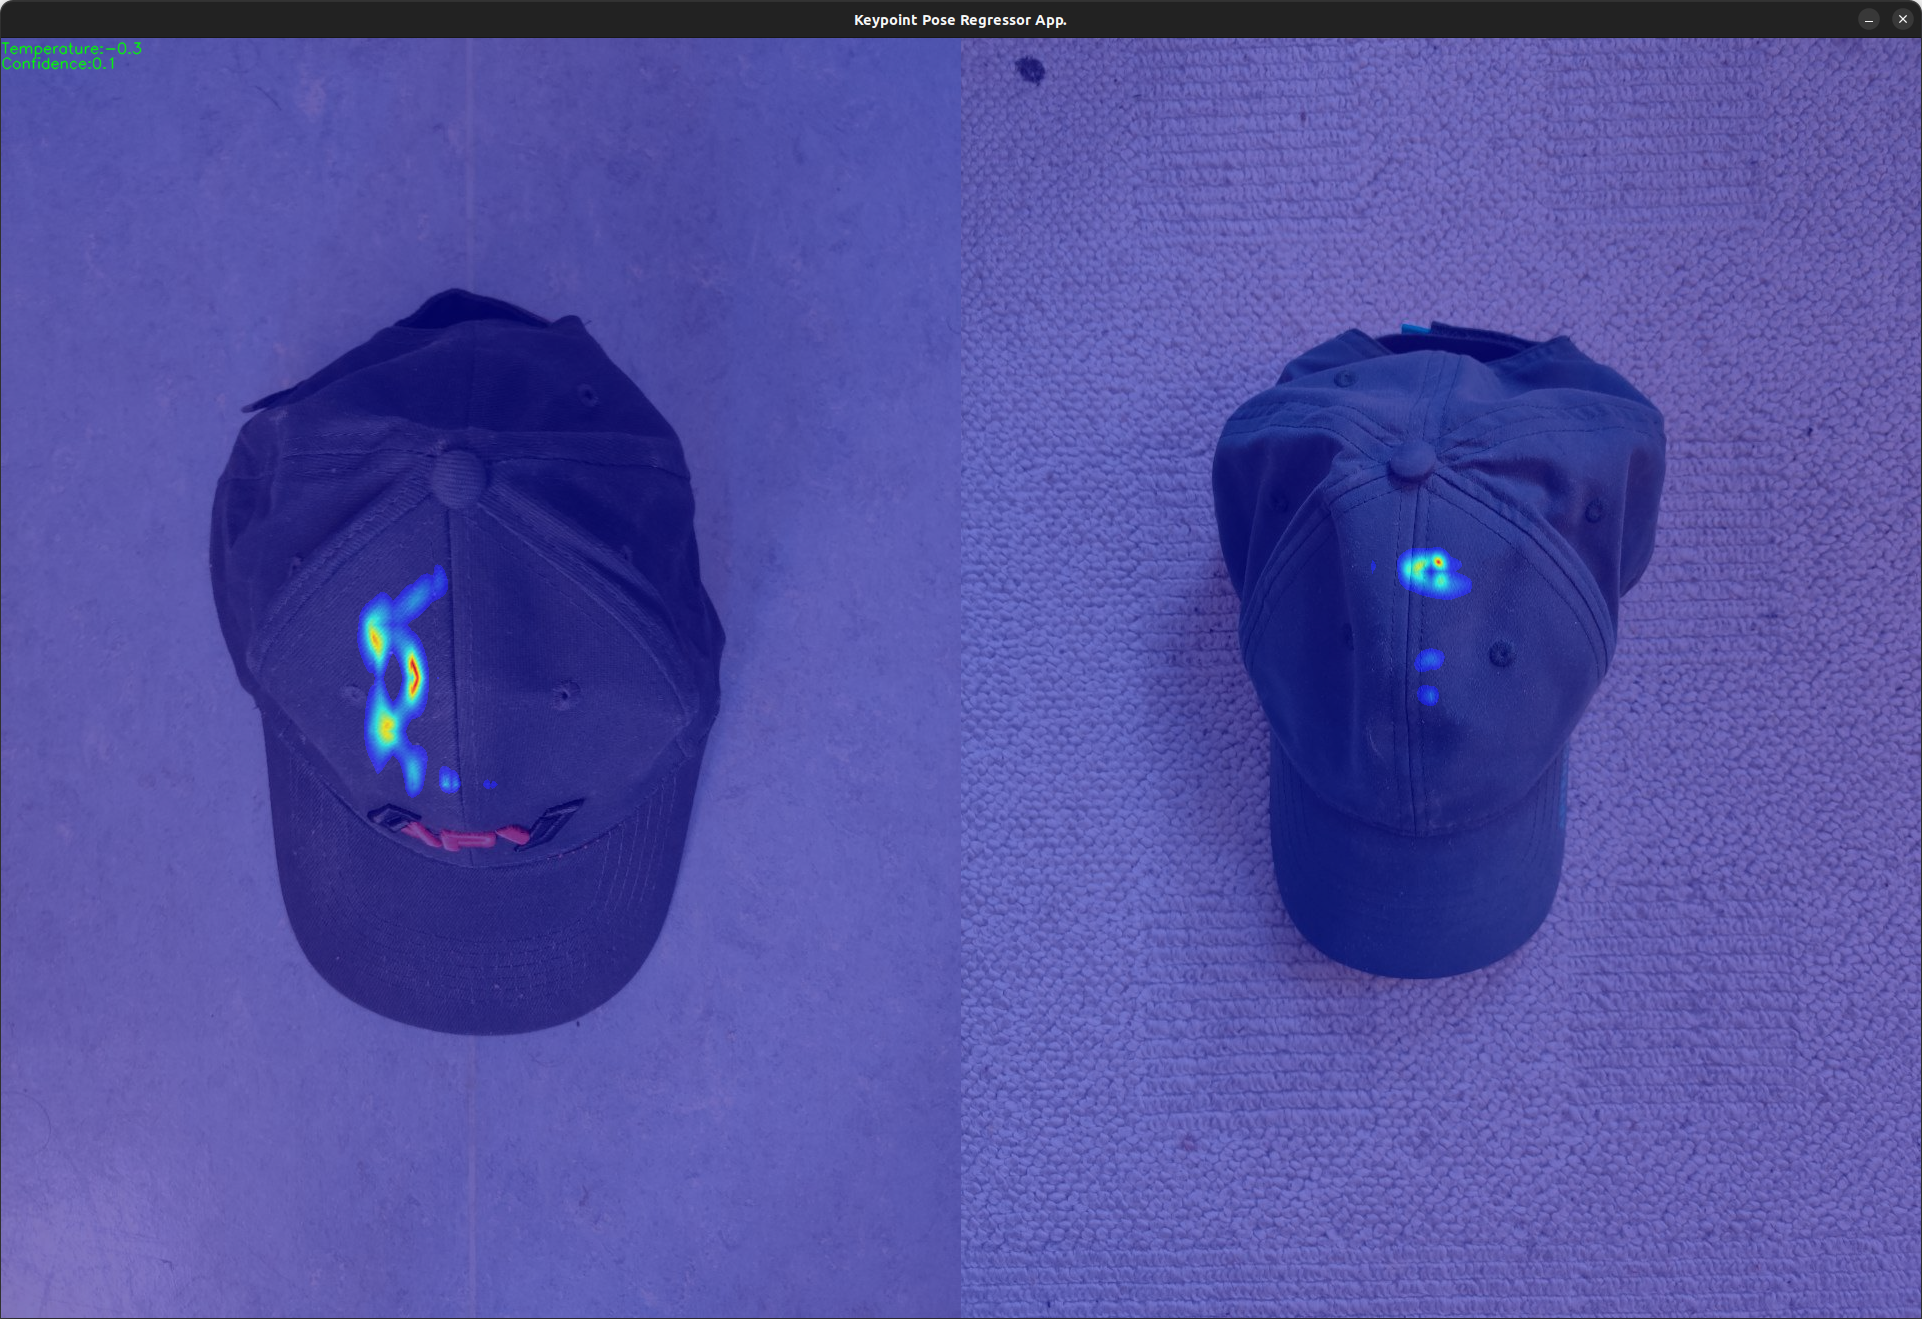
\includegraphics[scale=0.1]{images/cap/heatmaps.png}
\end{figure}

Furthermore, the \ac{DON} is testing using interactive application on the synthetic dataset.
As illustrated in the Figure~\ref{fig:don_performing_optimally} in page~\pageref{fig:don_performing_optimally}, the \ac{DON} performs optimally. The \ac{DON} places spatially optimal descriptors semantically across the objects in the same class.\\

\begin{figure}[htb]
    \centering
    \caption{\ac{DON} performing optimally on the synthetic dataset}
    \label{fig:don_performing_optimally}
    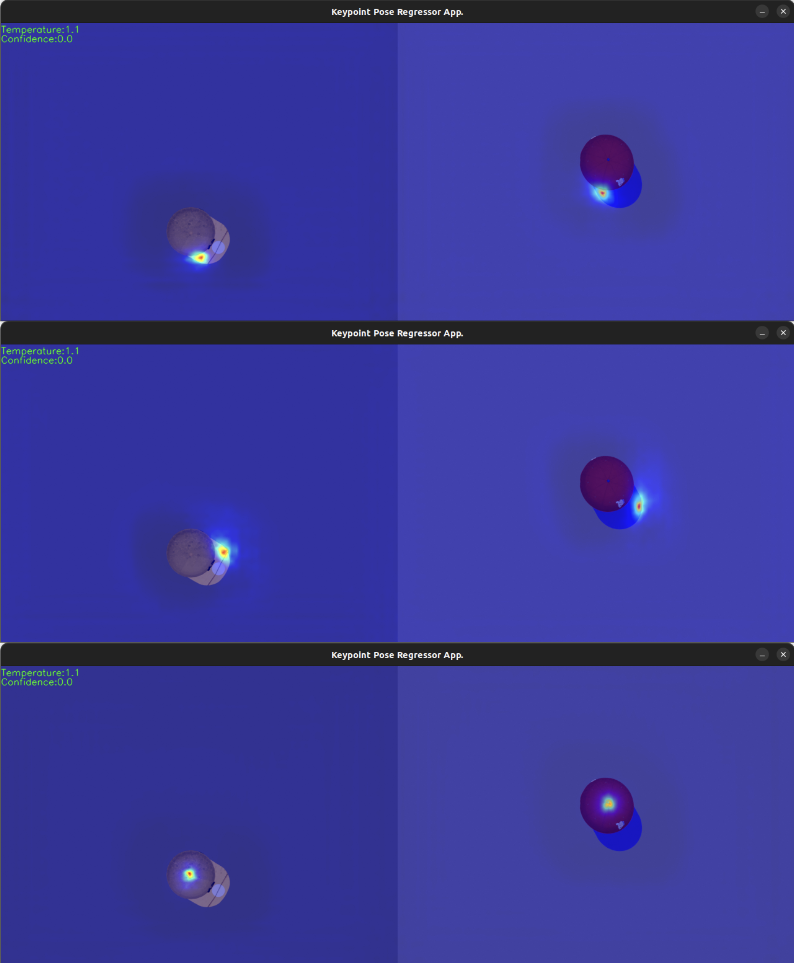
\includegraphics[scale=0.25]{images/cap/heatmaps_dataset.png}
\end{figure}

The synthetic dataset is perfect without any faults compared to the real-world data. Despite using background randomizations, noisy backgrounds, colour jitters and greyscaling augmentations, the \ac{DON} performs poorly on the real-world data as the
descriptors are not placed spatially optimally in the semantically same objects.

\subsection{\emph{``Not losing hope on the real world''}}

As per the results, the neural networks perform optimally locally in synthetic data and not real data, further posing an issue for robot grasping.\\

The neural network implementation scheme has three parts i.e., semantic correspondence mapping pipeline, \ac{DON} and KeypointNet to pick auto labels.
As the semantic correspondence pipeline is noisy and converged with errors as highlighted in Table~\ref{table:revised_benchmark_semantic_correspondence} in page~\pageref{table:revised_benchmark_semantic_correspondence},
the method of generating synthetic correspondences are adopted from \cite{adrian2022efficient} to train \ac{DON}. Furthermore, the \ac{DON} informed KeypointNet is adapted to regress
three keypoints on \ac{DON} representations generating geometrically consistent 6D poses.\\

To compute synthetic correspondences, the spatial grid $\mathcal{G}$ as in Equation \ref{eqn:spatial_grid} in page~\pageref{eqn:spatial_grid} is stacked
with the \ac{RGB} image such that the image dimension is as follows:

\begin{equation}
    I \rightarrow \mathbb{R}^{H \times W \times \mathbf{5}}
\end{equation}

Furthermore, the image is affinely augmented with previously used augmentations from the vision library provided by \cite{paszke2019pytorch}. Correspondences are the intersection of the spatial grid in the augmented image and the anchor image as illustrated in the Figure~\ref{fig:synthetic_correspondences}
in page~\pageref{fig:synthetic_correspondences}. These synthetic correspondences are further consumed to train \ac{DON}.

\begin{figure}[htb]
    \centering
    \caption{Illustrations of synthetic correspondences computed from the image augmentation. The pixel annotated in blue in the left image corresponds to the same pixel annotated in green in the right image.}
    \label{fig:synthetic_correspondences}
    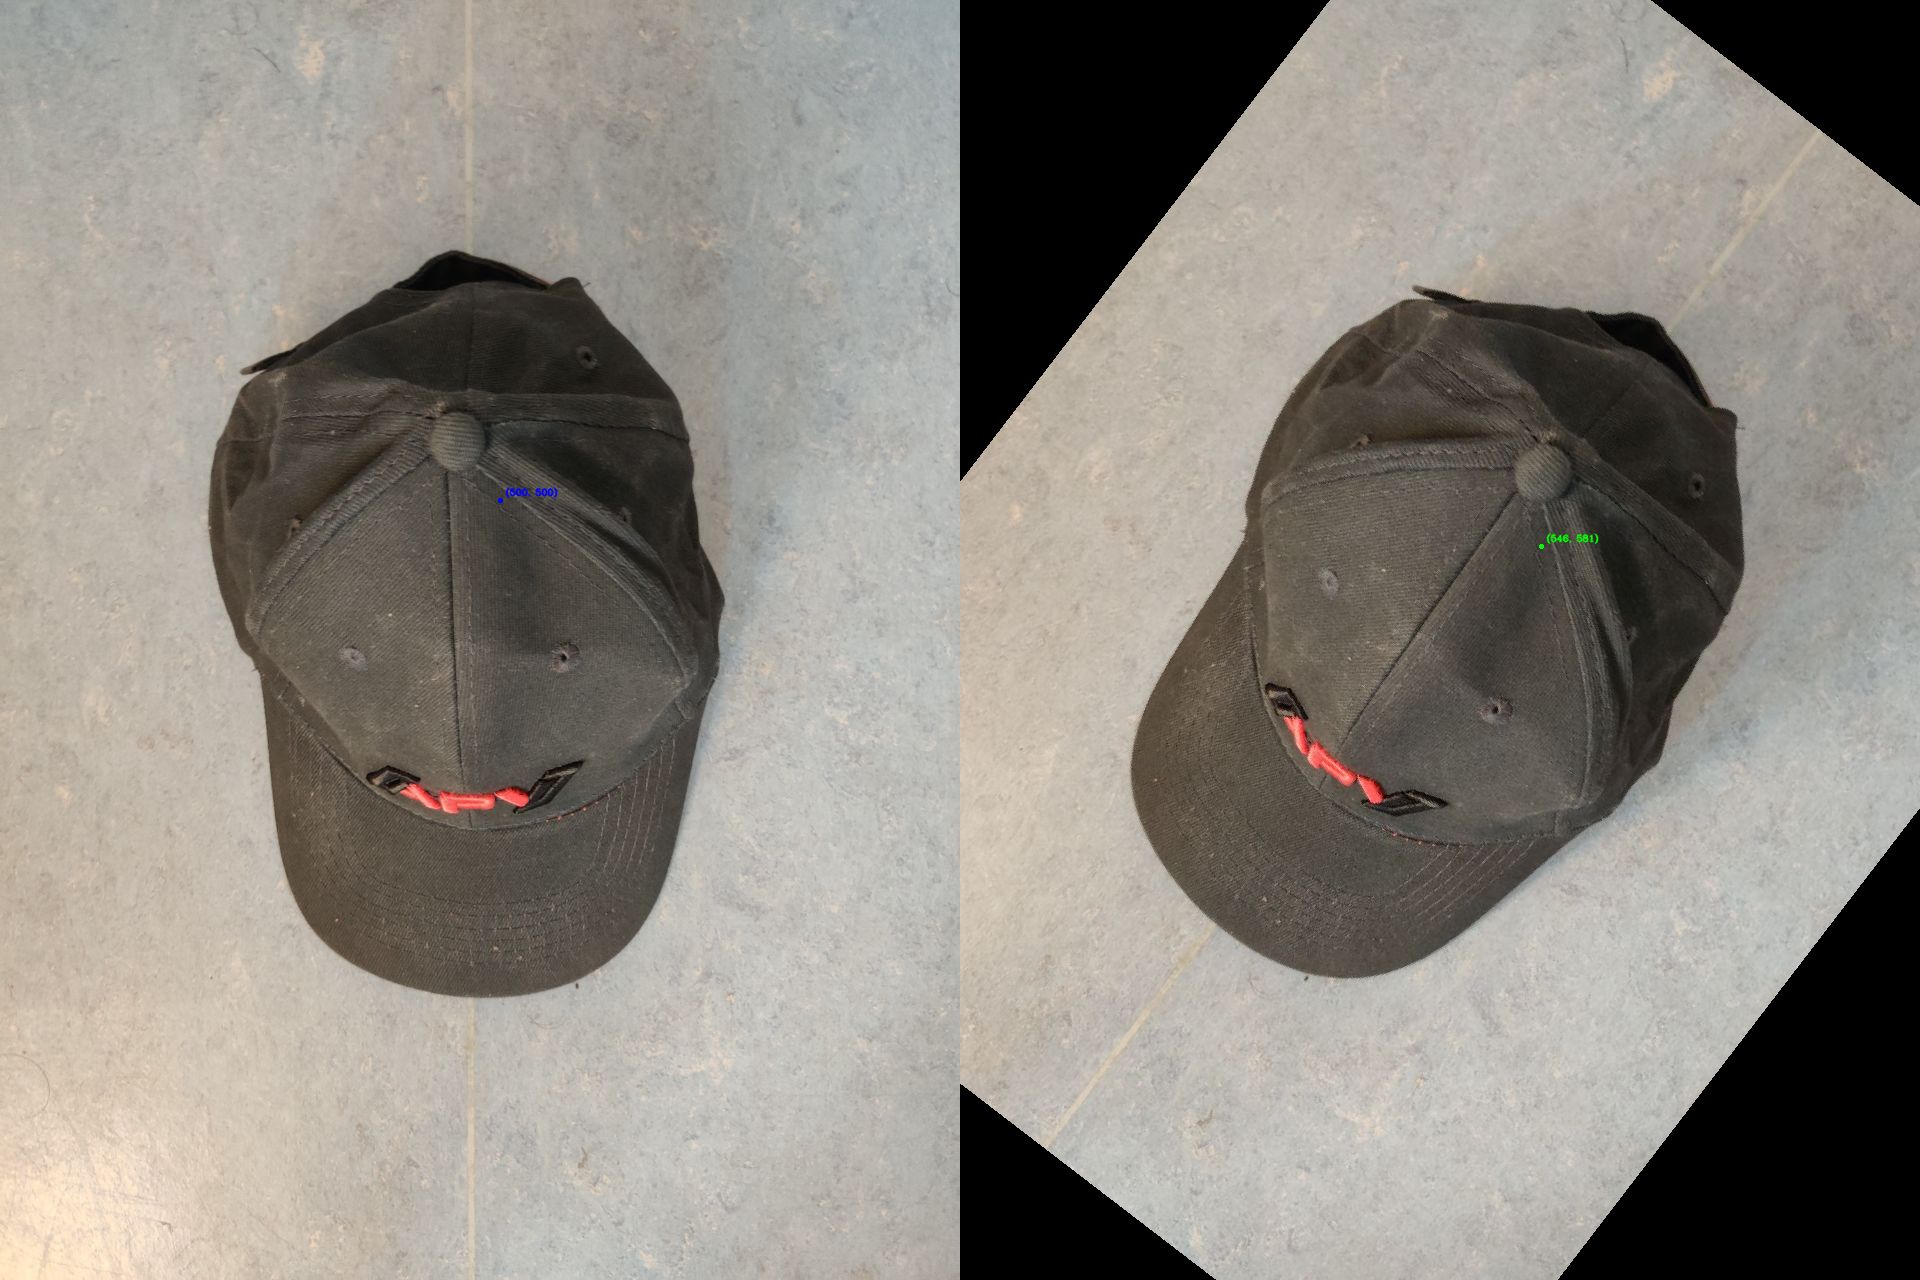
\includegraphics[scale=0.1]{images/cap/aug_image.png}
\end{figure}

The synthetic correspondences generalize caps in the real world pretty well, as depicted in the Figure~\ref{fig:real_heatmaps} in page~\ref{fig:real_heatmaps}.

\begin{figure}[htb]
    \centering
    \caption{Visual inspection of \ac{DON} trained on synthetic correspondences.}
    \label{fig:real_heatmaps}
    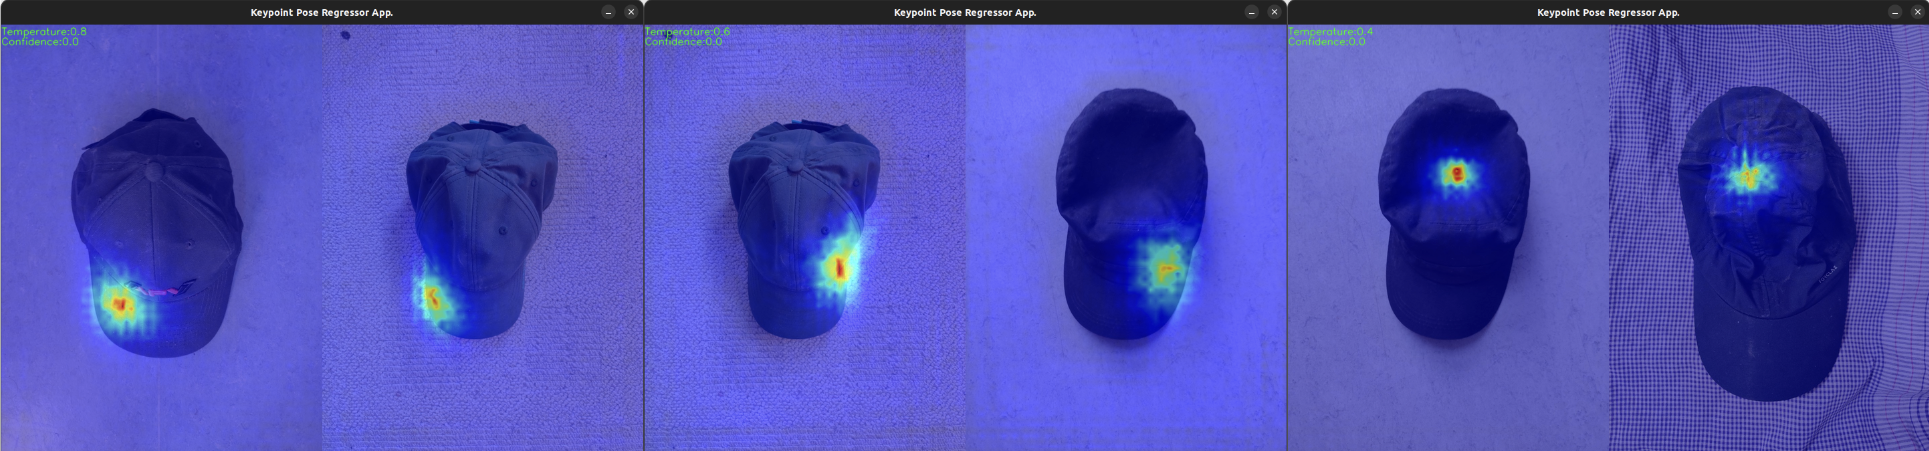
\includegraphics[scale=0.2]{images/cap/real_heatmap.png}
\end{figure}


\subsection{Robot Grasping Pipeline}

The KeypointNet is trained on the \ac{DON} representations to regress 3 geometrically consistent keypoints on dense descriptor images. These keypoint locations are the location of the dense descriptor labels.
Furthermore, these labels are stored offline in the .json format as rendered in the Listing~\ref{lst:json} in page~\pageref{lst:json}
for querying the descriptors in the real-time application.

\begin{lstlisting}[language=json, firstnumber=1, caption=Preview of json file entry of offline stored descriptors., label={lst:json}]
    ["cap":{
            "labels":[
                [3.1030, -3.4000, 2.9119],
                [5.2890, -2.5363, -0.7921],
                [0.0596, -3.8049, 2.1469]
            ]
            "priority":[
                1,
                2,
                3
            ]
        }
    ]
\end{lstlisting}

Both \ac{DON} and \ac{DON} informed KeypointNet, networks compute robot grasping poses as described below.

\subsubsection{Straight 3D Grasps with \ac{DON}}

As illustrated in Figure~\ref{fig:straight_grasp} in page~\pageref{fig:straight_grasp}, the robot moves to a position to capture the image of the cap. The \ac{RGB} image is fed into the \ac{DON} to compute a dense descriptor image.
The labels previously stored in .json format are read and extracted based on the priority to produce spatial expectation in the descriptor space.
The depth map is further used to project the spatial expectation and depth to camera coordinates for generating straight robot grasps.

\begin{figure}[htb]
    \centering
    \caption{3D grasping pipeline.}
    \label{fig:straight_grasp}
    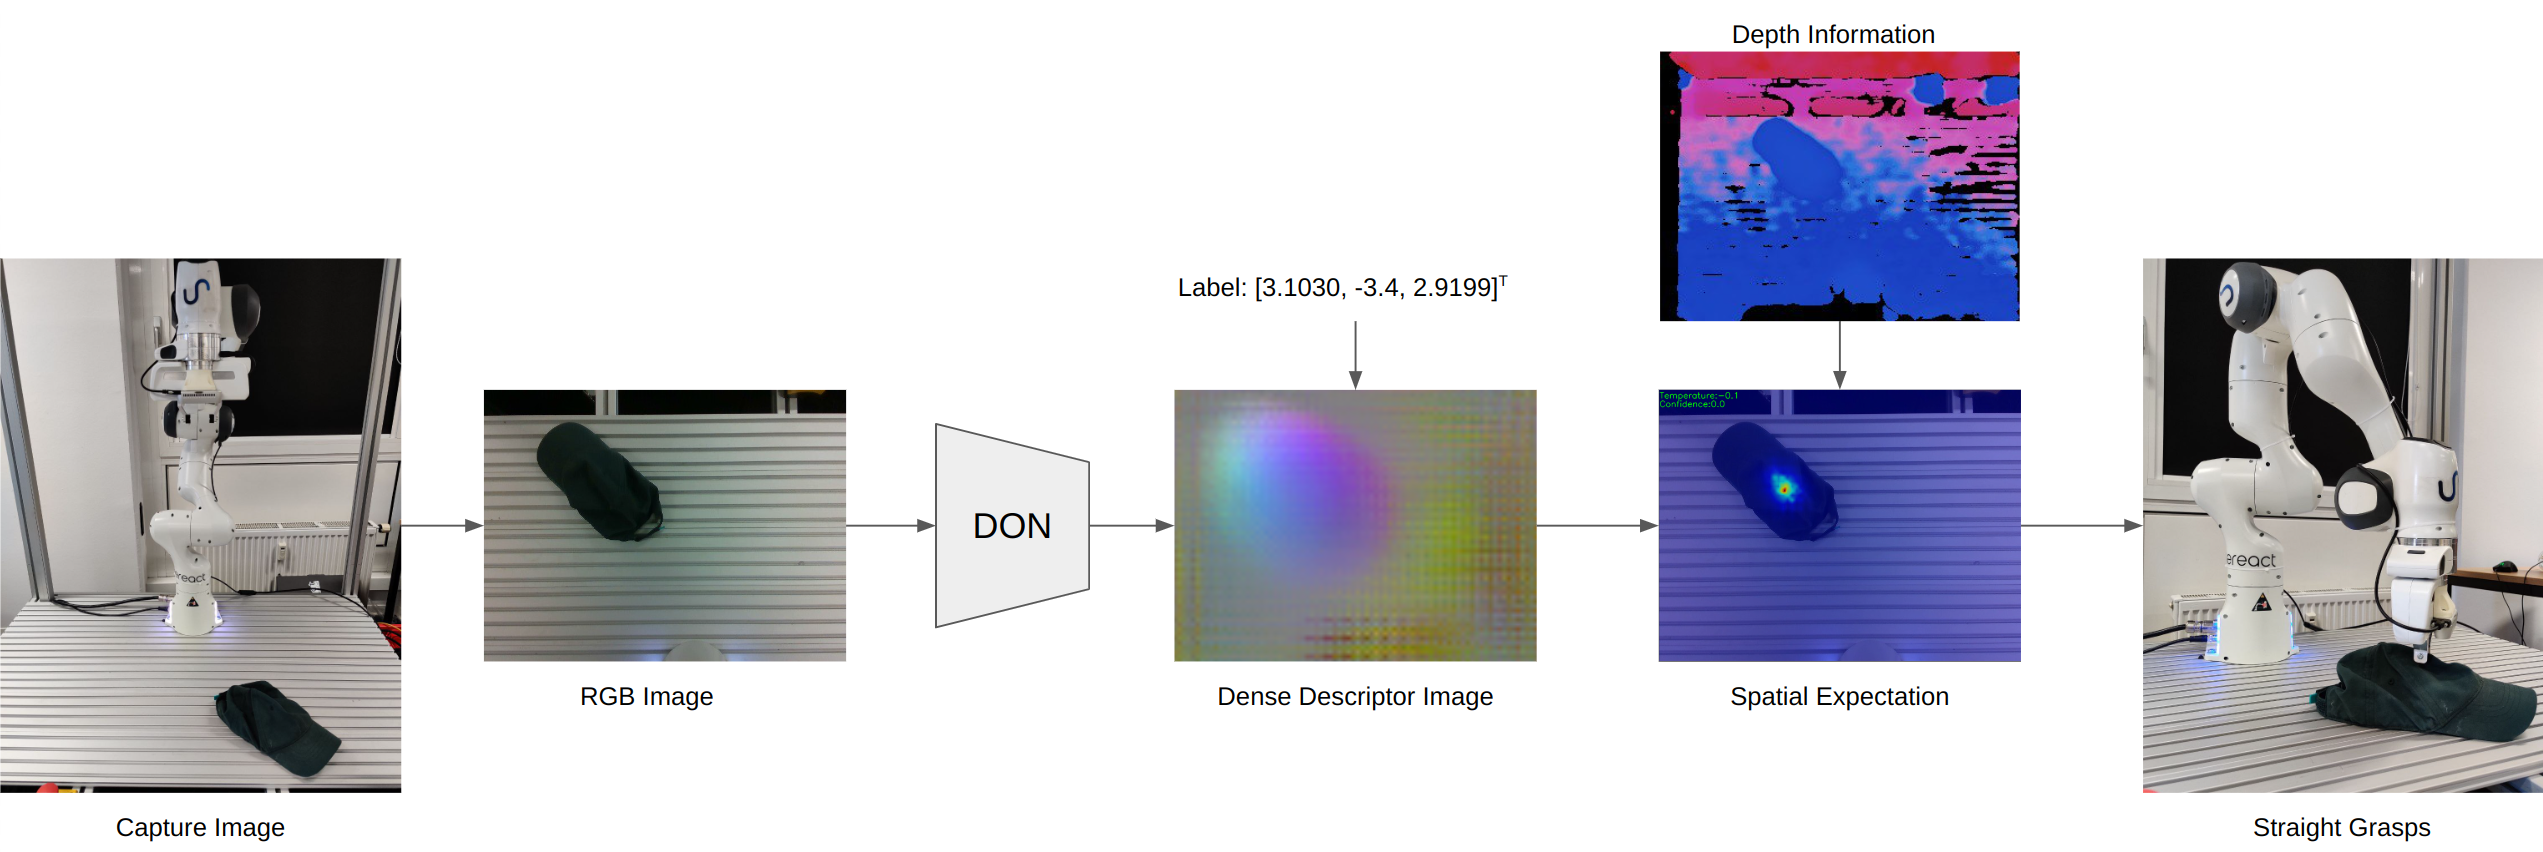
\includegraphics[scale=0.15]{images/robot/straight_grasps.png}
\end{figure}


\subsubsection{Aligned 6D Grasps with \ac{DON} Informed KeypointNet}

As depicted in Figure~\ref{fig:aligned_grasps}, the robot moves to a position to capture the image of the cap. The \ac{RGB} image is fed into the \ac{DON} Informed KeypointNet to compute object 6D pose. The robot
realigns the gripper according to the computed object 6D pose and, grasps the object.

\begin{figure}[htb]
    \centering
    \caption{6D grasping pipeline.}
    \label{fig:aligned_grasps}
    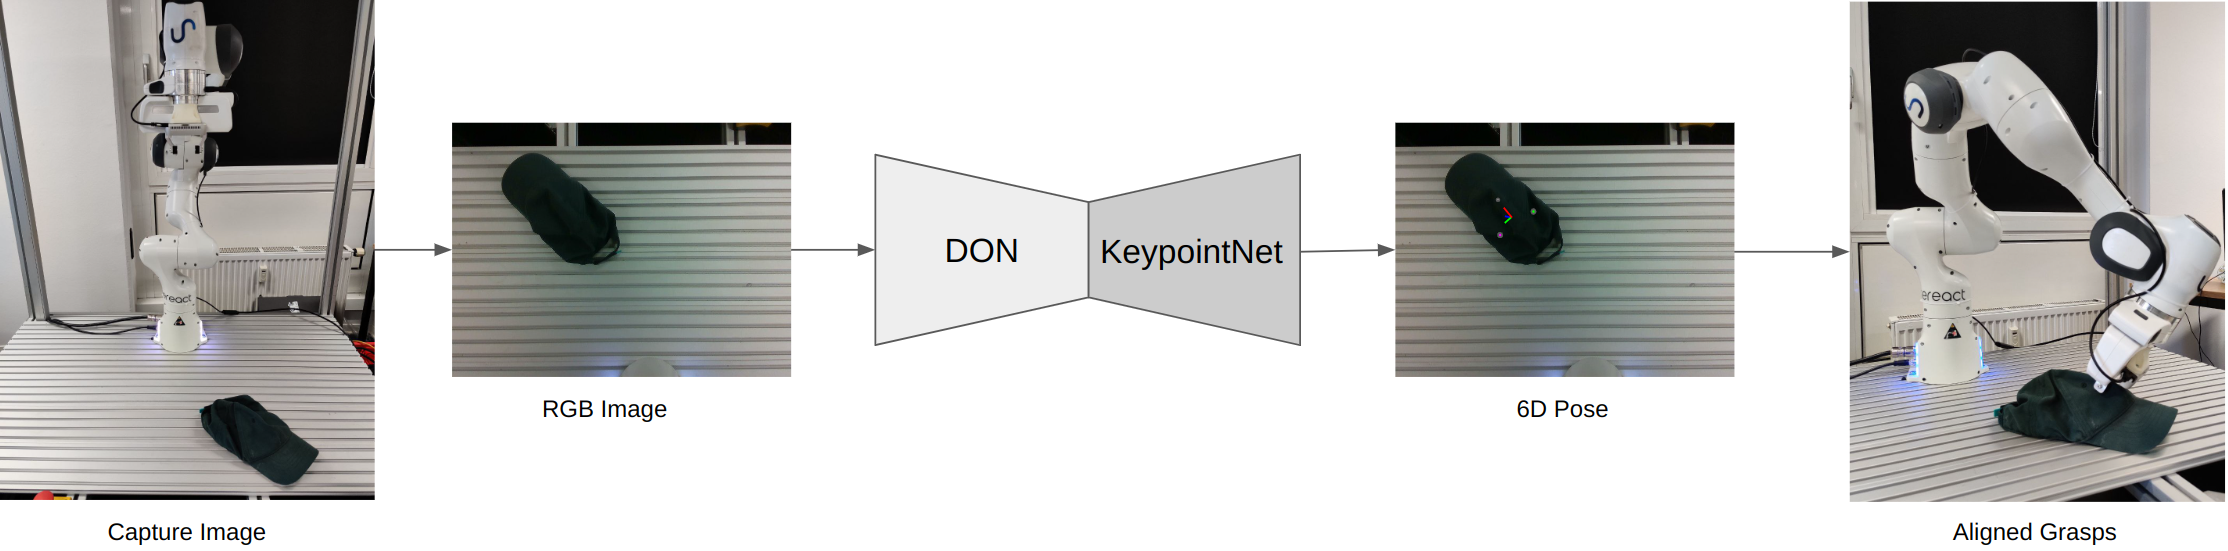
\includegraphics[scale=0.15]{images/robot/aligned.png}
\end{figure}

\subsubsection{Autonomous Robot Grasping Routine}

Figure~\ref{fig:complete_pipeline} depicts the autonomous robot grasping pipeline.
The robot consistently picks the cap robustly using both methods of generating grasps and places the caps aligned, mimicking the industrial robot palletizing routine effectively.

\begin{figure}[htb]
    \centering
    \caption{Autonomous robot grasping routine.}
    \label{fig:complete_pipeline}
    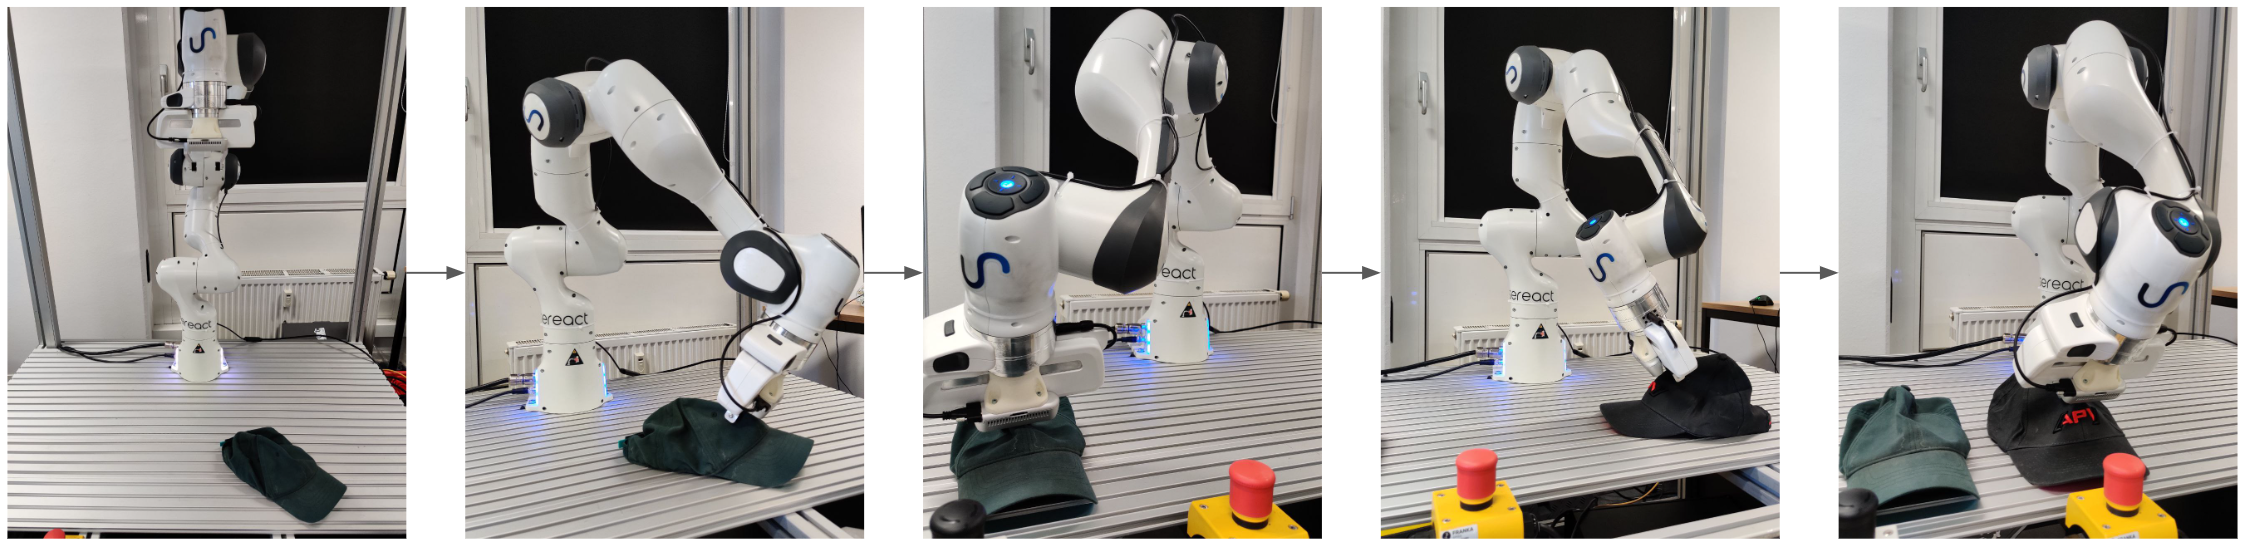
\includegraphics[scale=0.15]{images/robot/cycle.png}
\end{figure}